\chapter{Diode Rectifier Circuits}


\section{Objectives}
\begin{itemize}
    \item To verify a full-wave rectifier with center-tapped transformer
    \item To verify a full-wave bridge rectifier
\end{itemize}

\section{Materials}
\begin{itemize}
    \item Breadboard
    \item DC power supply
    \item Digital Multi-Meter
    \item \hyperref[1N4148]{Diode (1N4148)}
    \item Function Generator
    \item Oscilloscope
    \item Resistors
\end{itemize}

\section{Introduction}
In this experiment, we are going to learn the difference between two different kinds of full-wave diodes rectifier circuits. A function generator, resistors, and diodes will be used to construct the circuits, and an oscilloscope is used to observe and find the relationship between them.
     \subsection{Circuits}
        \begin{itemize}
            \item \textbf{Full-wave Diode Rectifier}\par
            Using the diode's characteristic of allowing current to flow in only one direction, it allows the diode circuit converting alternating current (AC) to direct current (DC) by depending on the half-cycle, specific diodes conduct to direct the current. It achieves this by utilizing both the positive and negative halves of the AC waveform, making it more efficient than a half-wave rectifier, which only uses one half.

            \item \textbf{Center-Tapped and Bridge Full-wave Rectifier}\par
            First and for most, two full-wave rectifier require two different type of transformer. And the number of diodes required to configure the circuit is different.\par
            Comparison:\par
            \begin{itemize}
                \item Center-Tapped Full-wave Rectifier uses two diodes, and a secondary winding is split into two equal halves with a center tap that serves as the reference point. The AC input is applied across the two halves of the secondary winding, and each diode conducts during one half of the AC cycle, producing a full-wave rectified output.
                \item Bridge Full-wave Rectifier uses four diodes. During both halves of the AC input cycle, two of the four diodes conduct, ensuring that current flows in the same direction through the load, providing a full-wave rectified output.
            \end{itemize}
            Consumption:\par
            \begin{itemize}
                \item Center-Tapped Full-wave Rectifier outputs DC voltage is approximately the peak voltage of the transformer secondary minus the diode threshold voltage ($V_{peak}$ - $V_\gamma$).
                \item Bridge Full-wave Rectifier outputs DC voltage is approximately the peak voltage of the transformer secondary minus the diode build-in voltage, $V_{peak}$ - 2$V_\gamma$ (since two diodes conduct in each half-cycle).
            \end{itemize}
        \end{itemize}
        
    \subsection{Circuit Diagram}
        \begin{figure}[h]
            \centering
            \begin{subfigure}[h]{0.45\textwidth}
                \centering
                \includesvg[width=0.95\linewidth]{Lab03/Lab3a.drawio.svg}
                \caption{}
                \label{Lab3a}
            \end{subfigure}
            \hfill
            \begin{subfigure}[h]{0.45\textwidth}
                \centering
                \includesvg[width=0.95\linewidth]{Lab03/Lab3b.drawio.svg}
                \caption{}
                \label{Lab3b}
            \end{subfigure}
        \end{figure}
        \FloatBarrier
    The resistor shown in Fig.\ref{Lab3a} and Fig.\ref{Lab3b} has the resistance of 1k$\Omega$, and diode used is \hyperref[1N4148]{1N4148}.
\section{Detailed Procedures}
We used oscilloscope to observe $V_o$, $V_{D_1}$ and $V_{D_2}$.\par
Full-wave diode rectifier with center-tapped  transformer:\par
    \begin{figure}[h]
        \centering
        \begin{subfigure}[h]{0.45\textwidth}
            \centering
            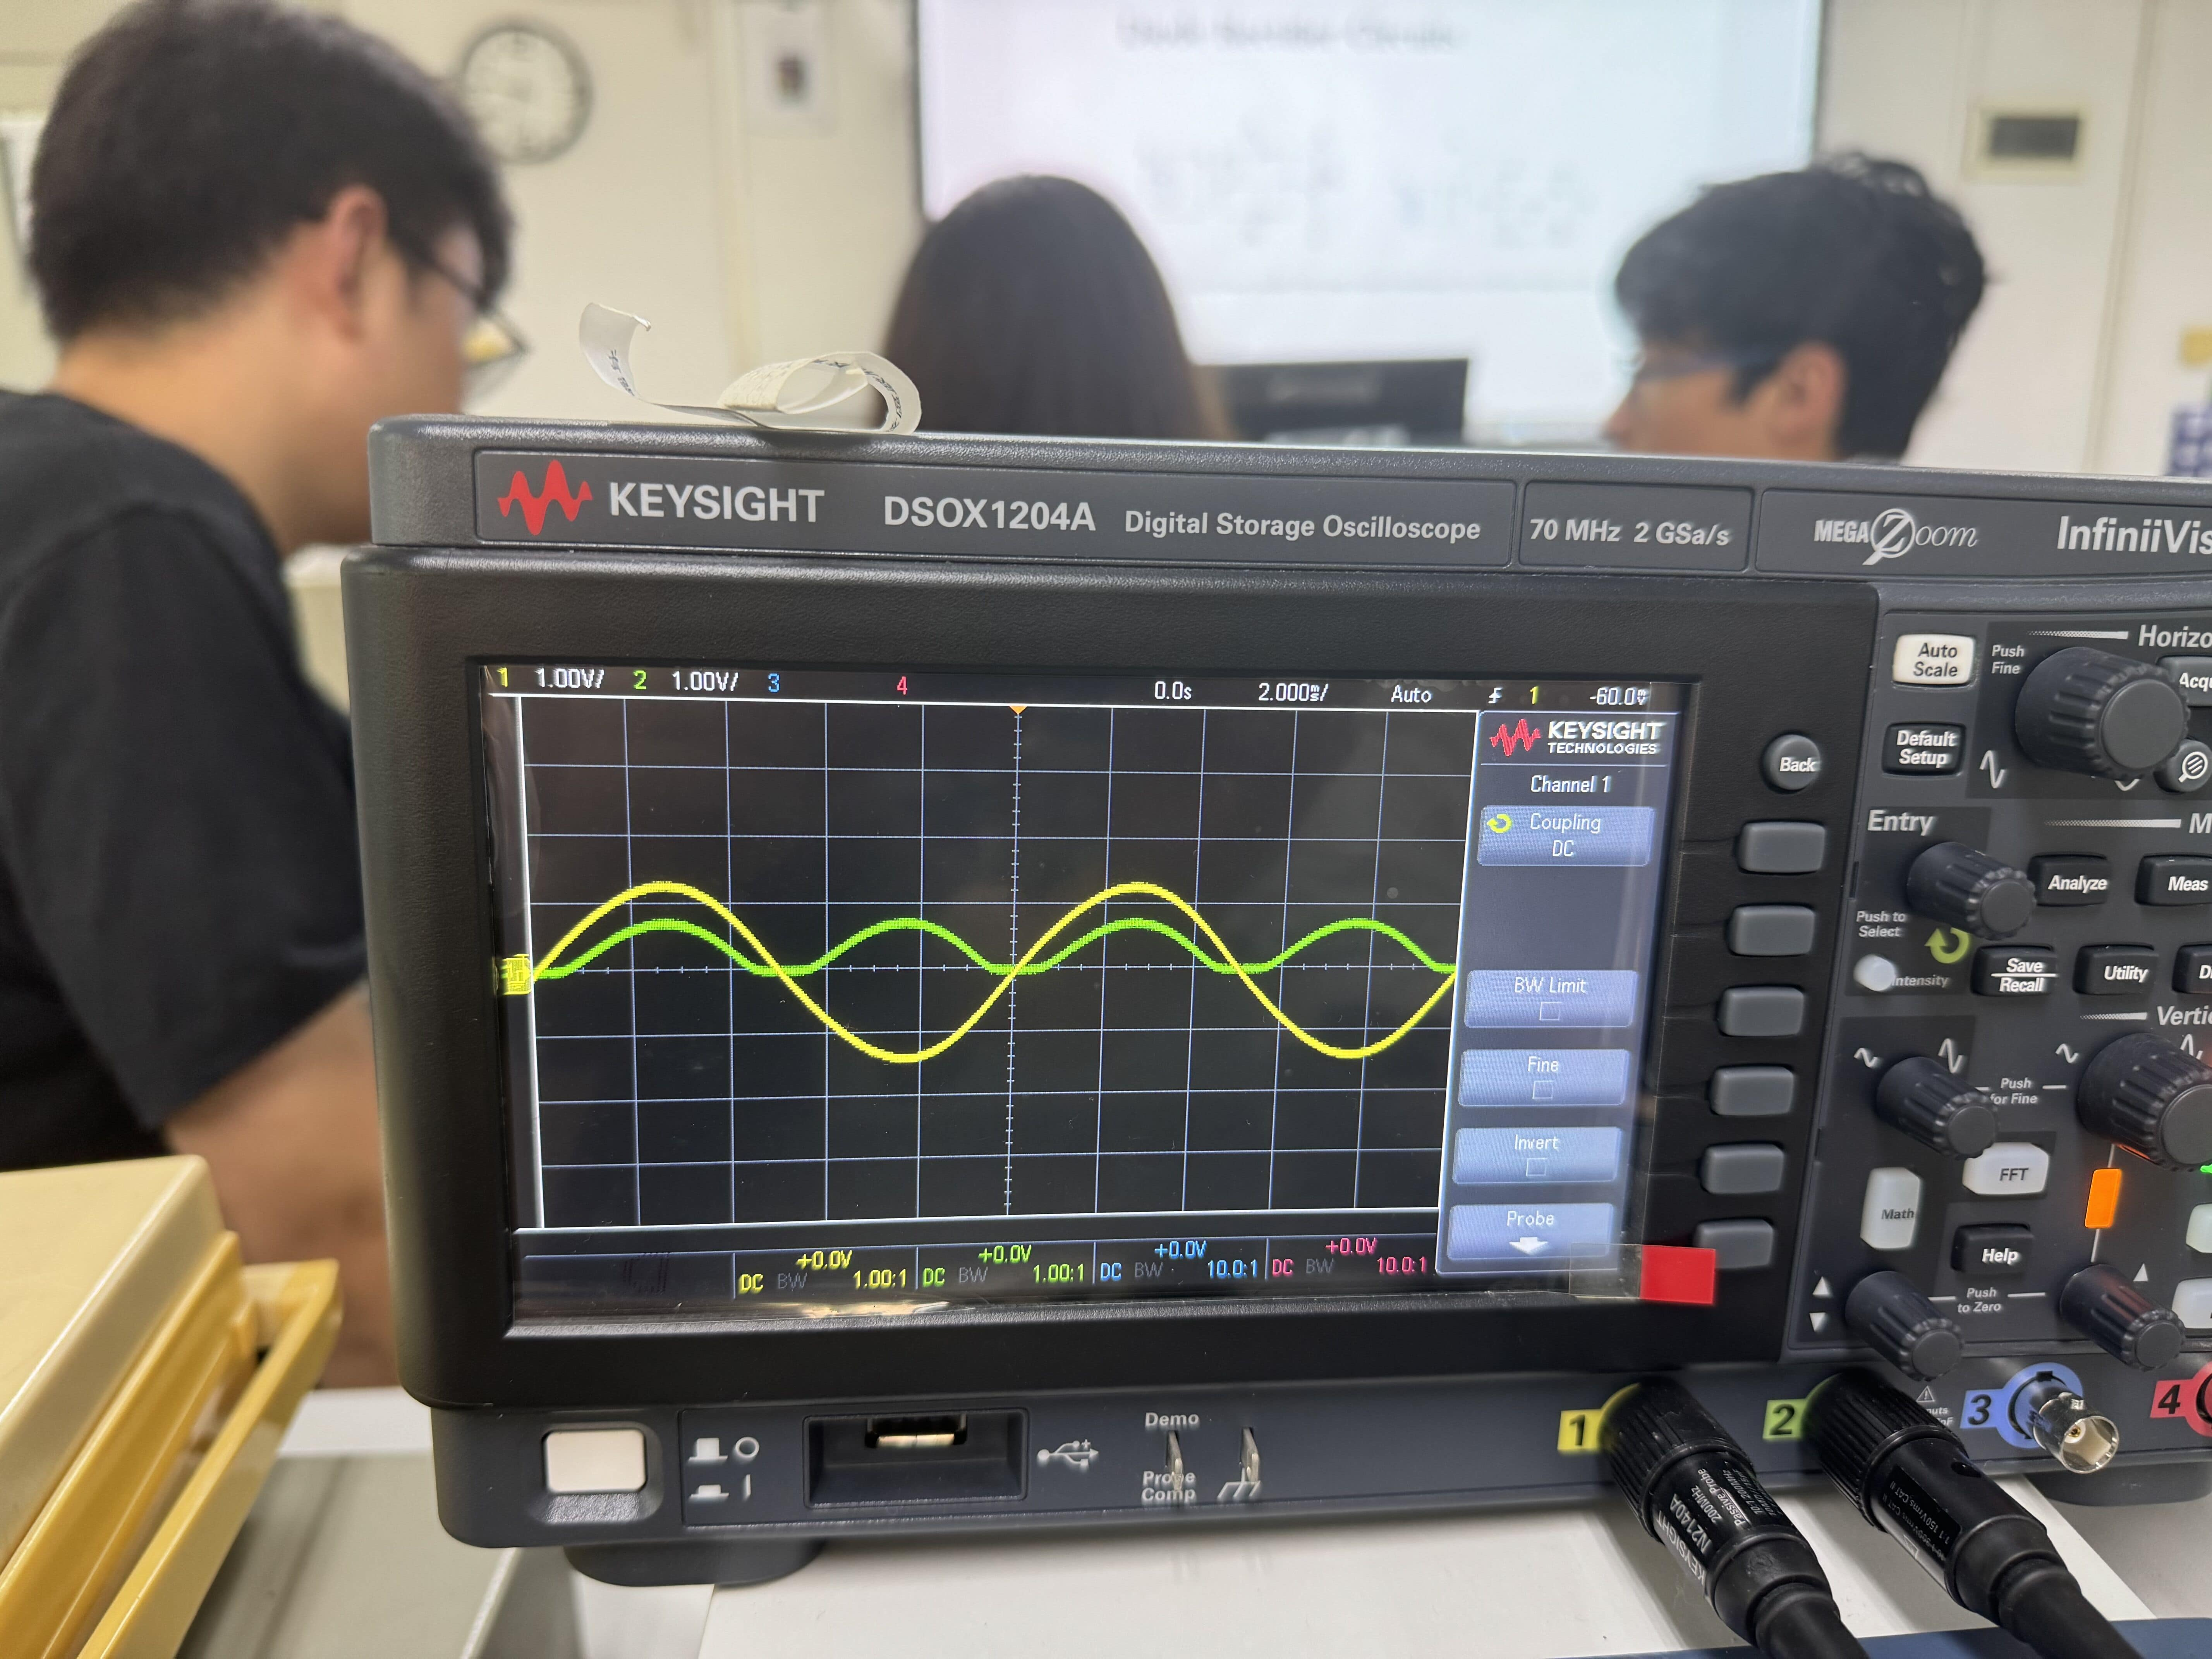
\includegraphics[width=0.9\textwidth]{Lab03/Images/3.4_outPutVoltage.jpg}
            \caption{Output Voltage}
            \label{L3.4OV}
        \end{subfigure}
        \hfill
        \begin{subfigure}[h]{0.45\textwidth}
            \centering
            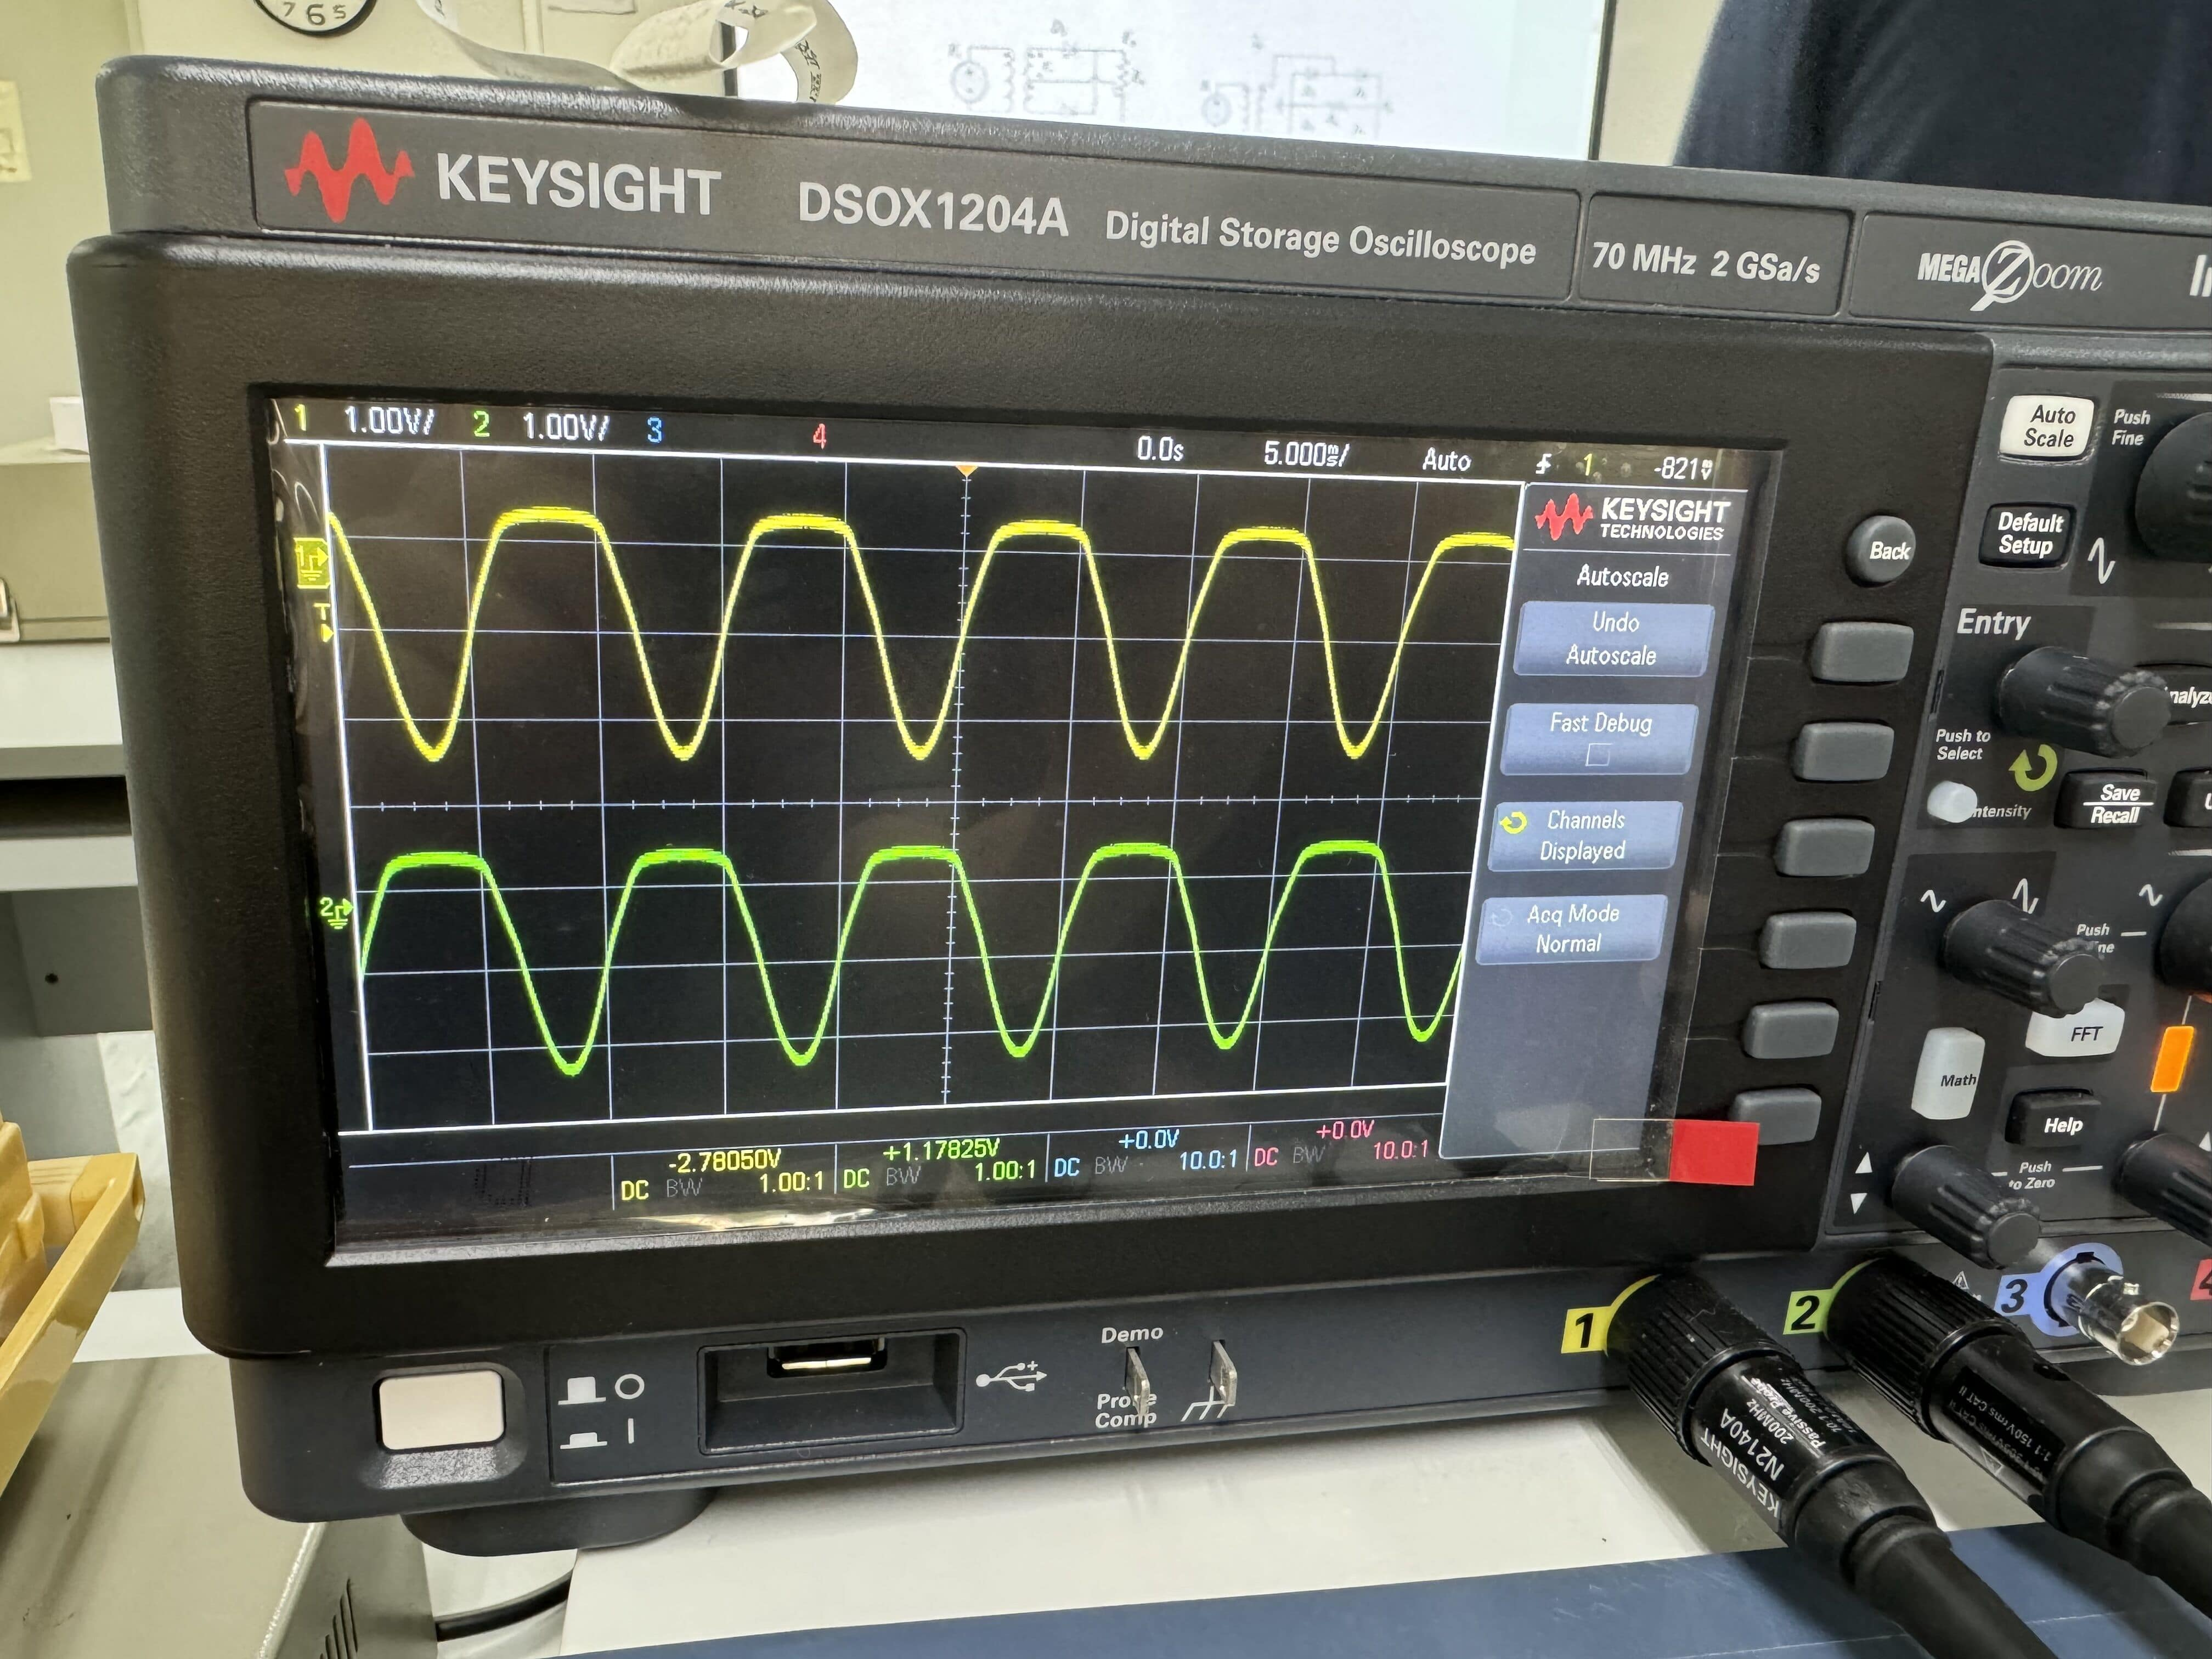
\includegraphics[width=0.9\textwidth]{Lab03/Images/3.4_diodeVoltage.jpg}
            \caption{Diode Voltage}
            \label{L3.4DV}
        \end{subfigure}
    \end{figure}
    \FloatBarrier
From Fig.\ref{L3.4OV}, we can see the $V_o$ flipped the negative signal to positive signal and has lower amplitude than $V_i$. And Fig.\ref{L3.4DV} shows the two diodes are alternatively working.

Full-wave bridge diode rectifier:\par
    \begin{figure}[h]
        \centering
        \begin{subfigure}[h]{0.45\textwidth}
            \centering
            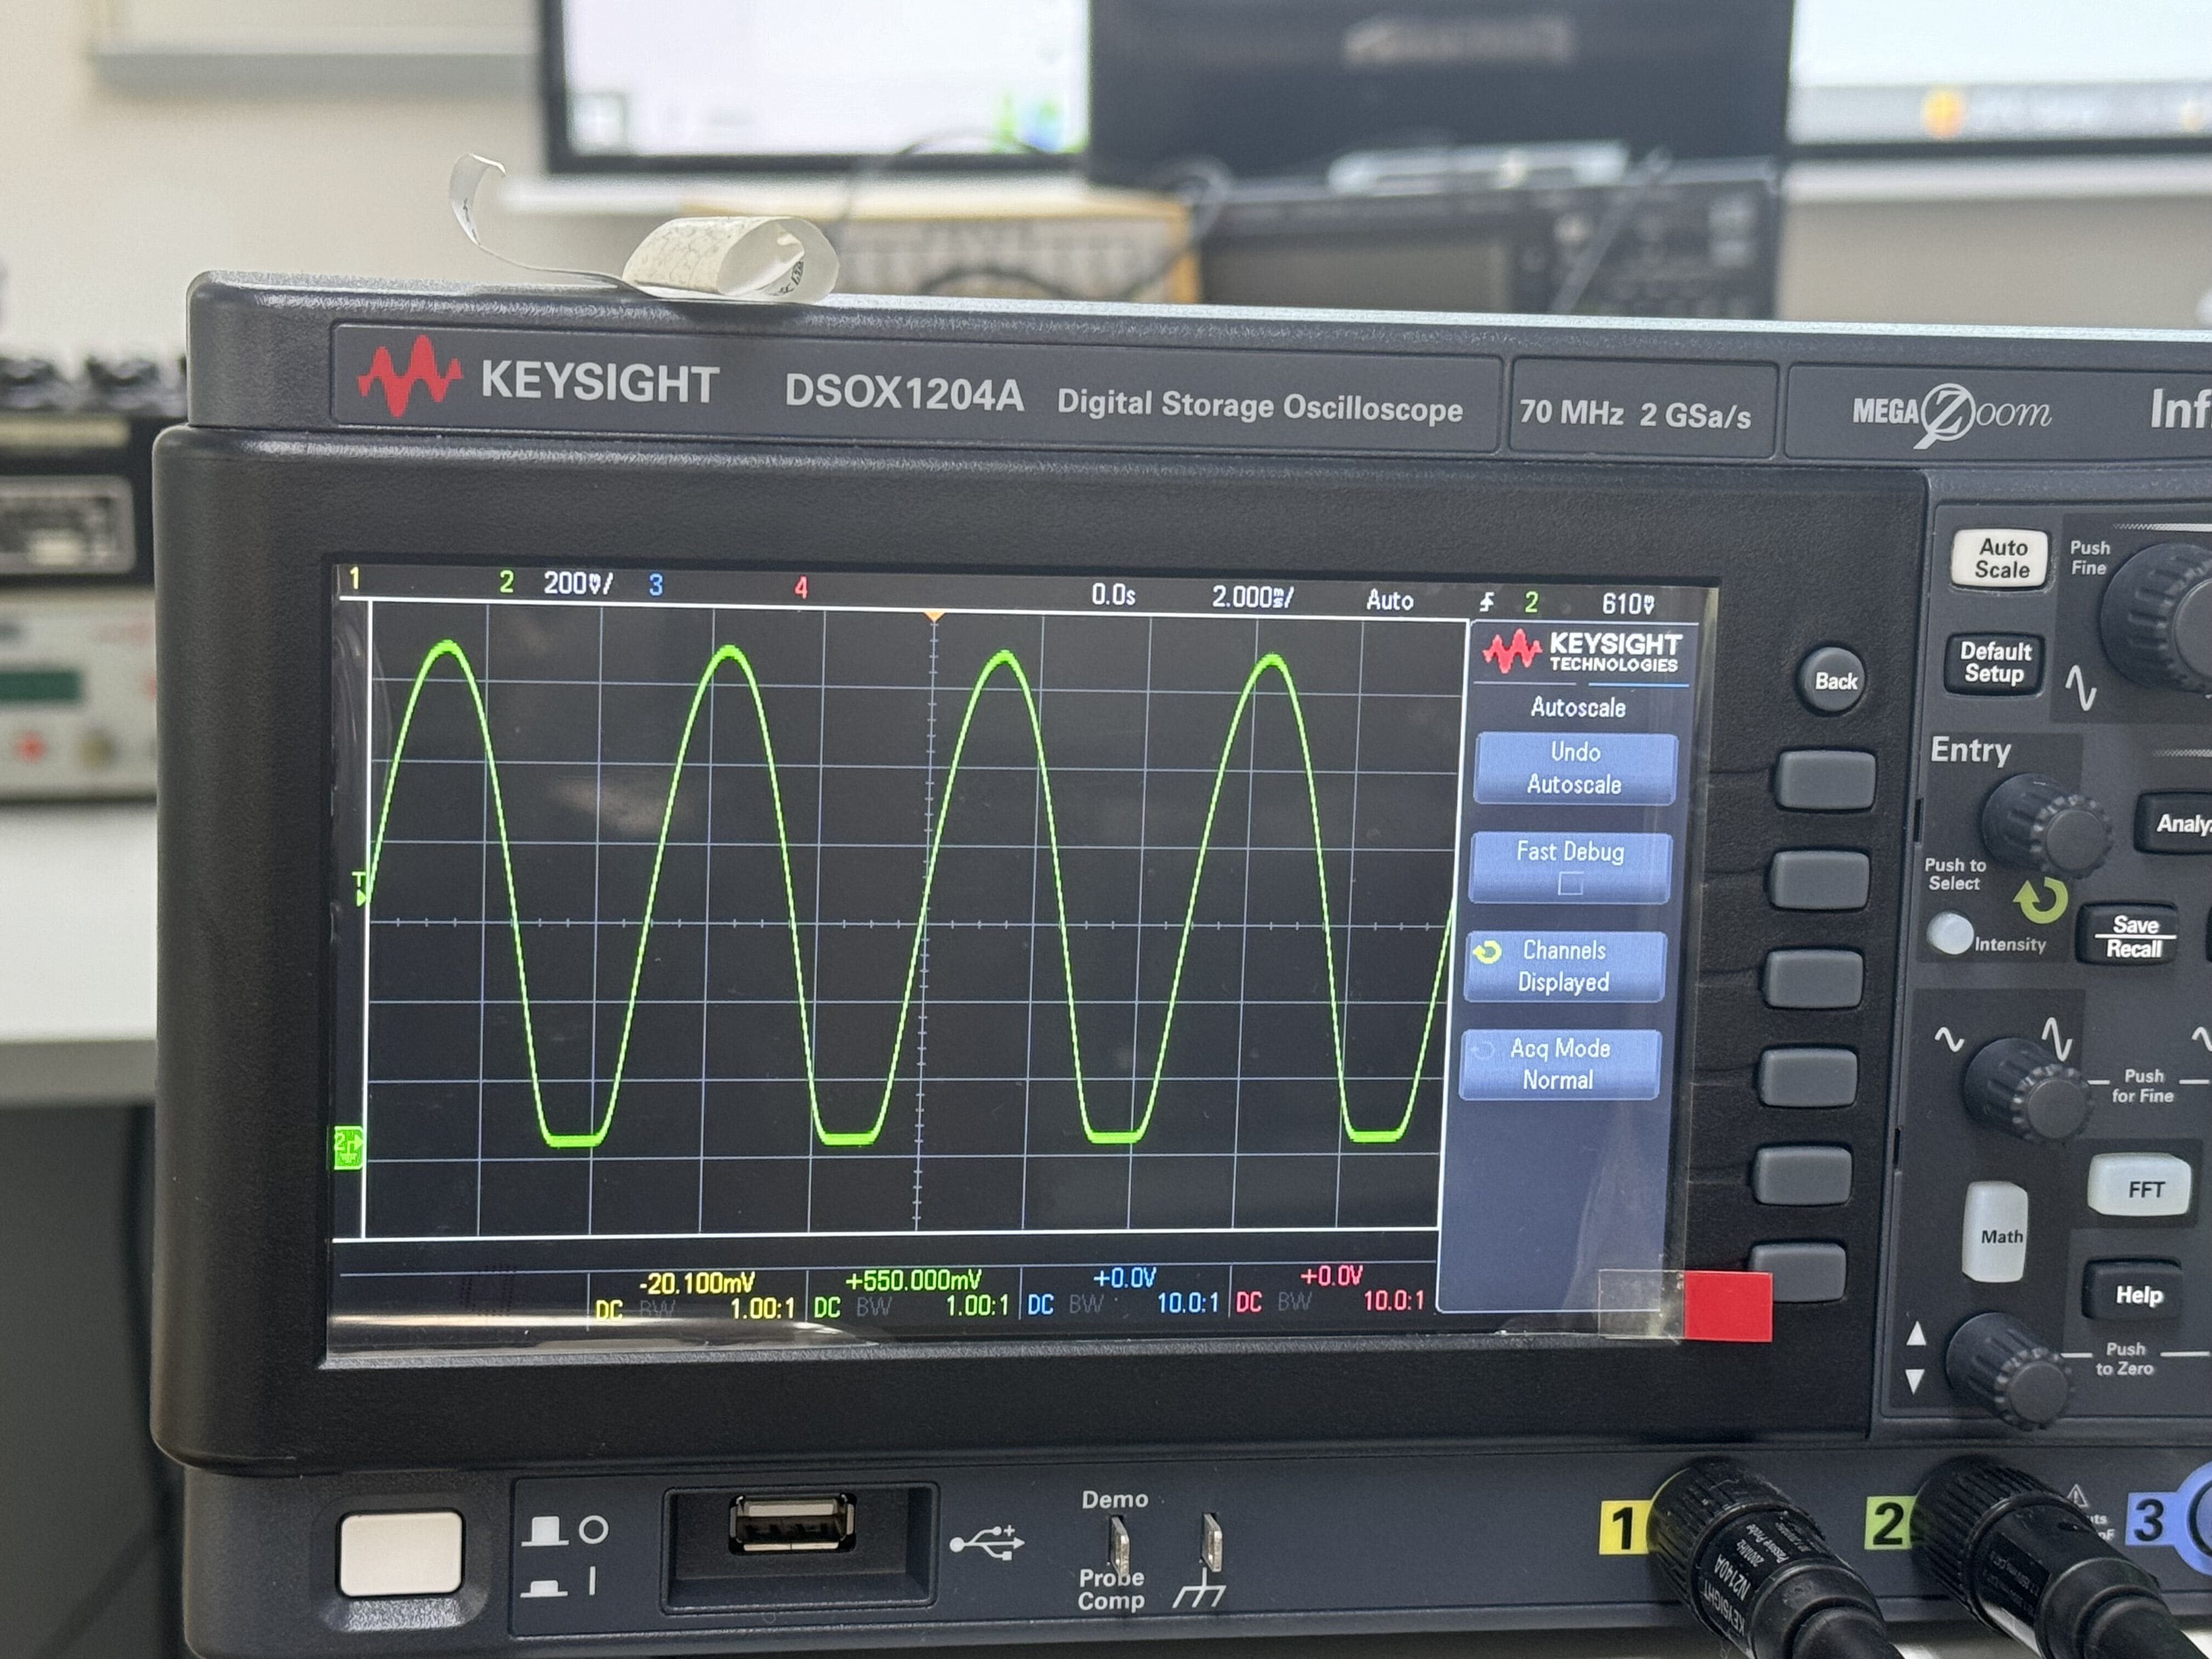
\includegraphics[width=0.9\textwidth]{Lab03/Images/3.5_outPutVoltage.jpg}
            \caption{Output Voltage}
            \label{L3.5OV}
        \end{subfigure}
        \hfill
        \begin{subfigure}[h]{0.45\textwidth}
            \centering
            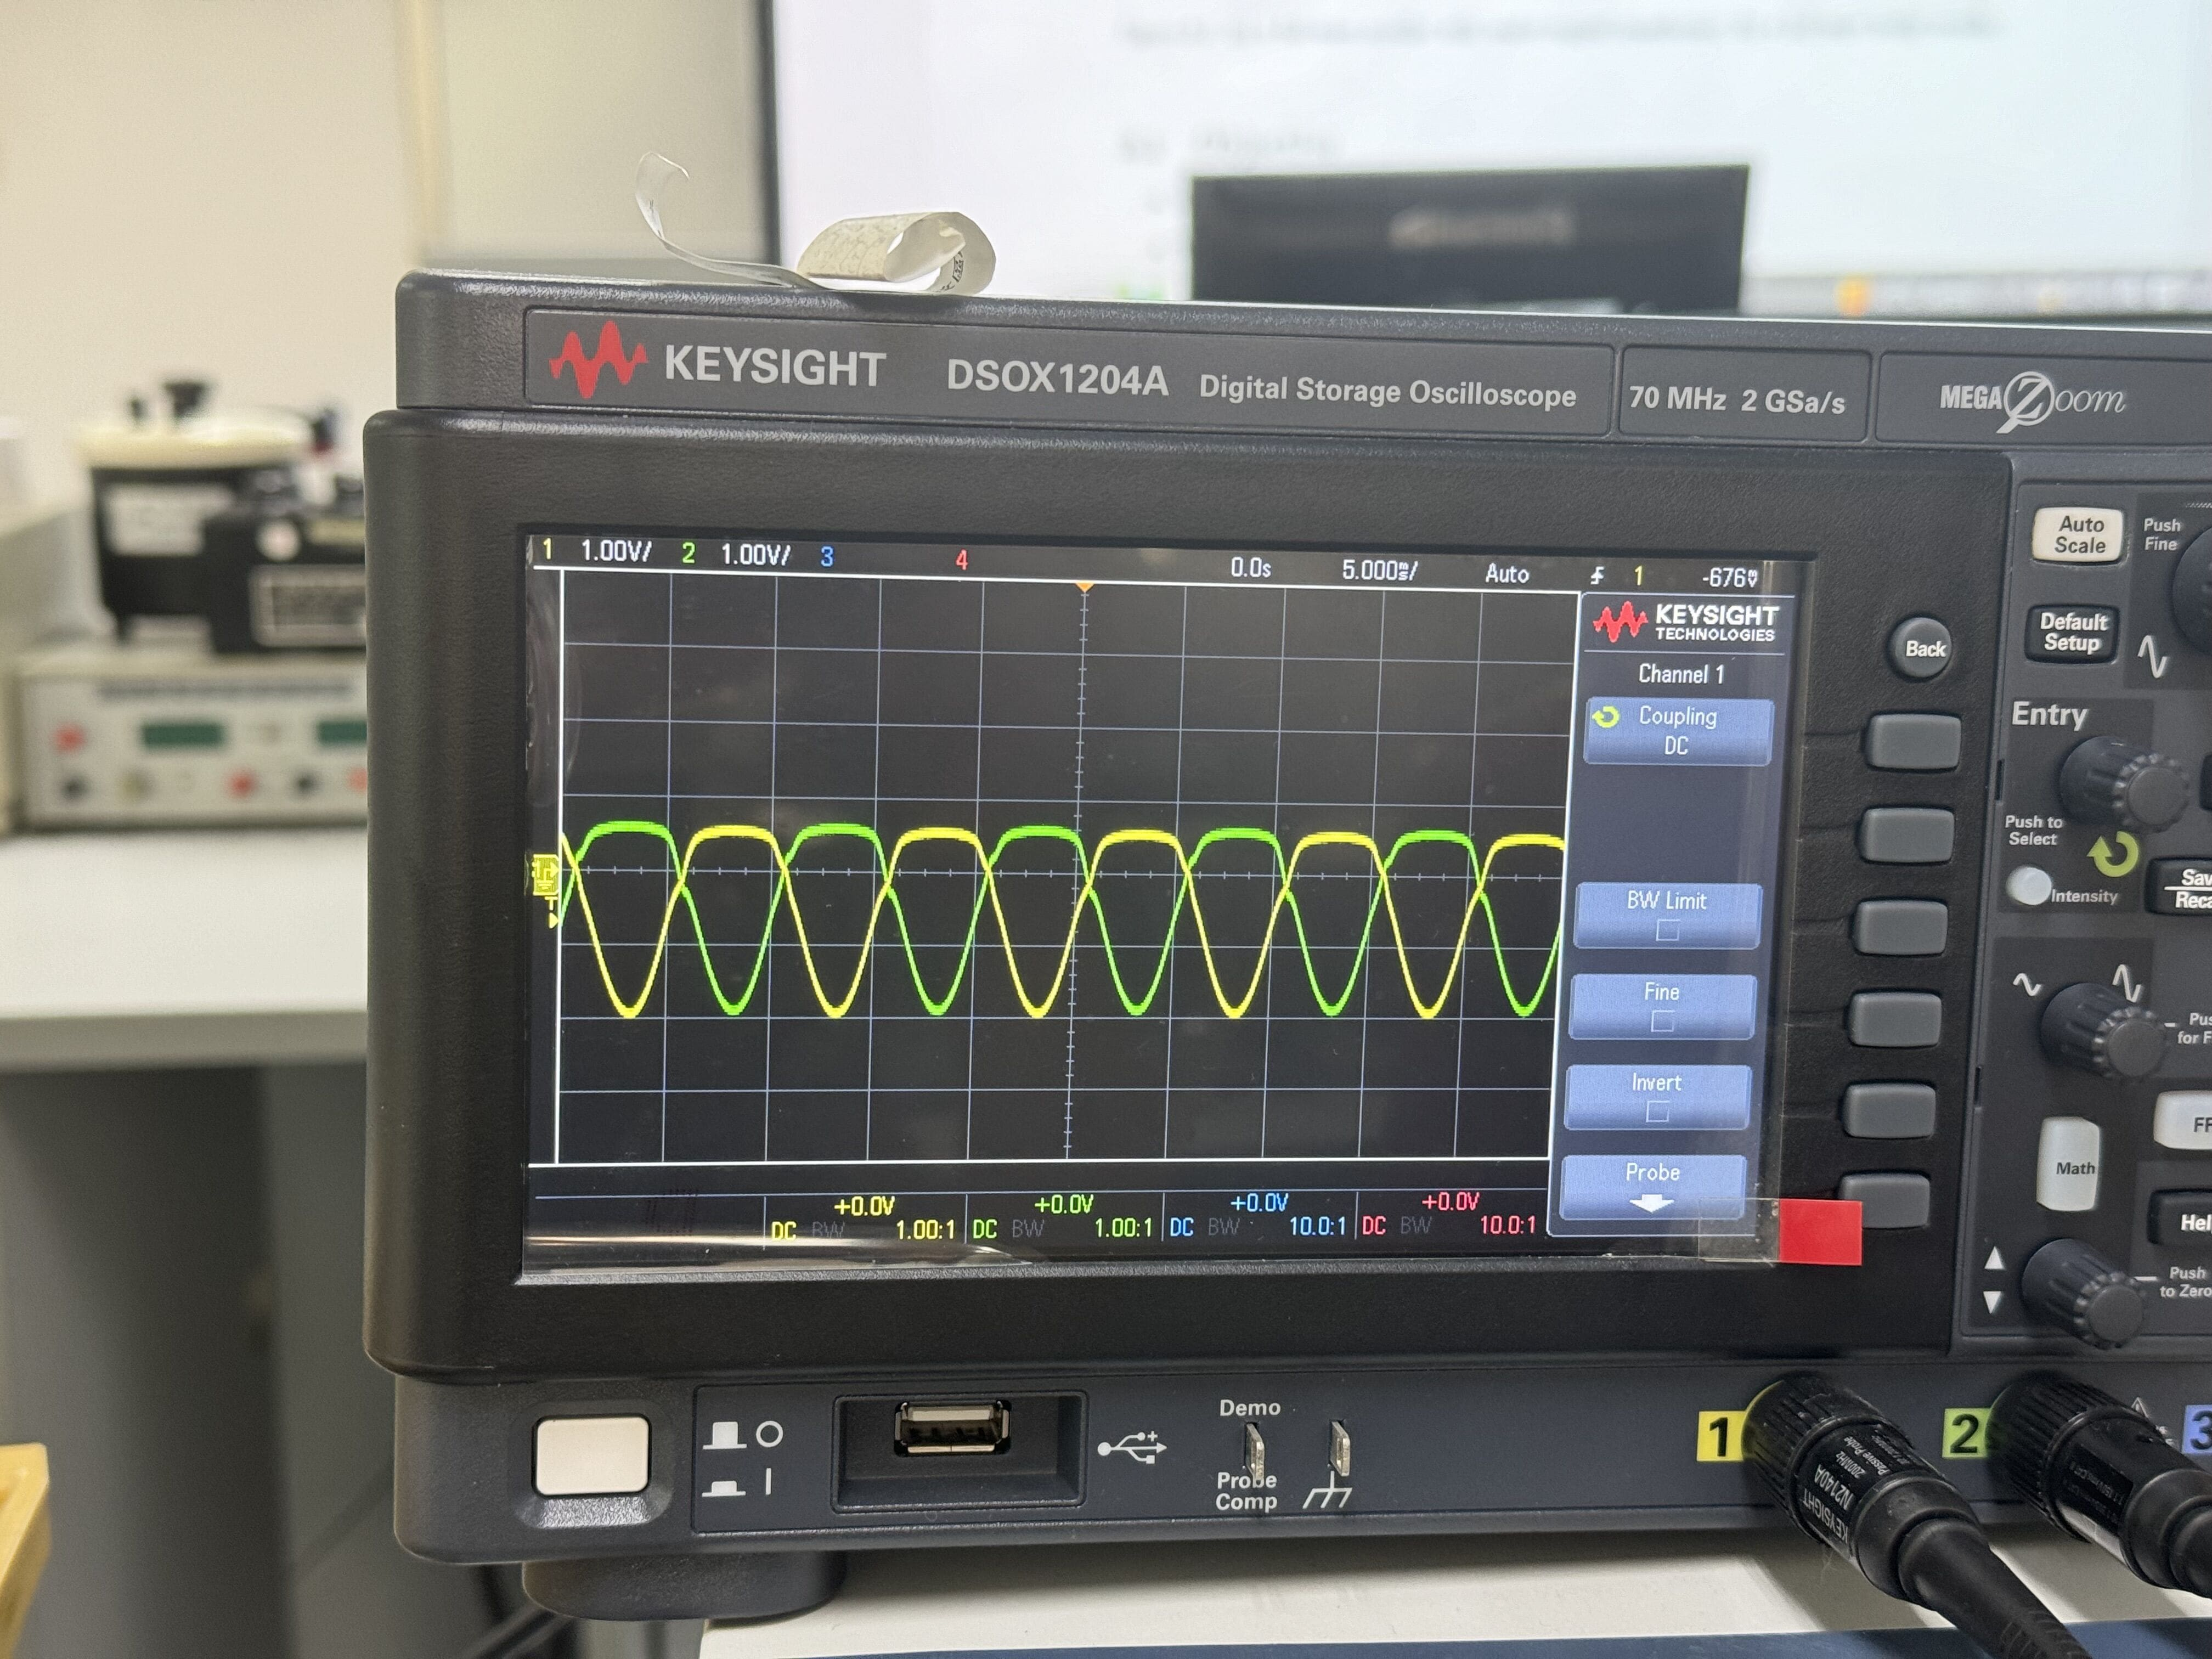
\includegraphics[width=0.9\textwidth]{Lab03/Images/3.5_diodeVoltage.jpg}
            \caption{Diode Voltage}
            \label{L3.5DV}
        \end{subfigure}
    \end{figure}
    \FloatBarrier
From Fig.\ref{L3.5OV}, we can see the $V_o$ has only positive signal and the amplitude is less than 3V. And Fig.\ref{L3.5DV} shows the two diodes are alternatively working.

\section{Discussion}
From the Figure.\ref{L3.4OV} we can tell the function generator did not output expected signal, the amplitude did not reach 3V. Therefore the observed output also is not the same as predicted.

\section{Conclusion}
In conclusion, the experiment reinforces the understanding of full-wave rectifiers. The bridge rectifiers are generally more versatile, efficient, and cost-effective for a wide range of applications. On the other hands, even though center-tapped rectifiers need less diodes which means less cost and dissipates less energy when it is rectifying, they require complex and expensive center-tapped transformer.